\subsection{Performance Results and Analysis}
\label{results}
Of tens of thousands of our sampling runs, we find that the fully populated
cases---i.e., both producer and consumer counts become equal to the total
process count---are most revealing. In particular, we carefully analyze 
the maximum latency of each of the main phases of KAP for these cases 
because this metric represents the critical path of the performance of
many HPC process management services. For example, distributed 
HPC software would use KVS operations in a coordinated fashion to exchange 
connection information among processes during its bootstrapping 
phase as shown in LIBI~\cite{LIBI} and PMI~\cite{PMI2}. Unless {\em all} 
of the distributed processes complete their
KVS operations, their communication fabric cannot be established. 

\begin{figure}
  \centering
  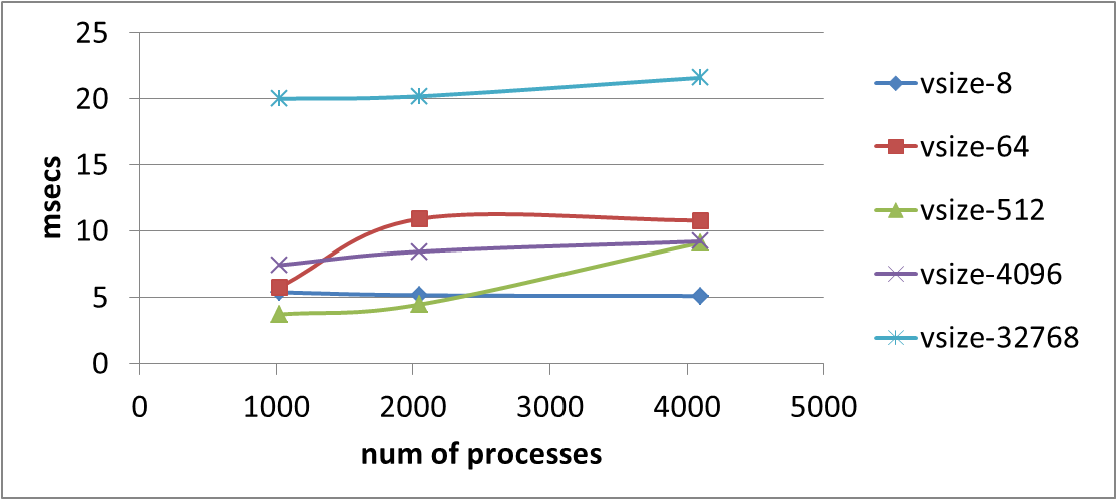
\includegraphics[width=1.0\linewidth]{producer}
  \caption{Max latency of producer phase}
  \vspace{-.4cm}	
  \label{fig:prod}
\end{figure}

Figure~\ref{fig:prod} shows the maximum latency of the producer phase.
Essentially, these plots indicate how well {\tt kvs\_put}
scales as we increase the number of producers. Each plot represents
different value sizes---e.g., {\tt vsize-8} refers to value size being
8 bytes. As shown in this graph, the {\tt kvs\_put} simply performs and
scales well. This matches our expectations because objects
are cached in write-back mode at {\tt kvs\_put} time and flushed to the
server at the next consistency event. 

%\ifcomments
%\marginpar{\tiny JG: The vsize-32768 requires some explanation}
%\fi
%
%\begin{figure}[ht]
%\centering
%\begin{subfigure}[With unique values]{
%  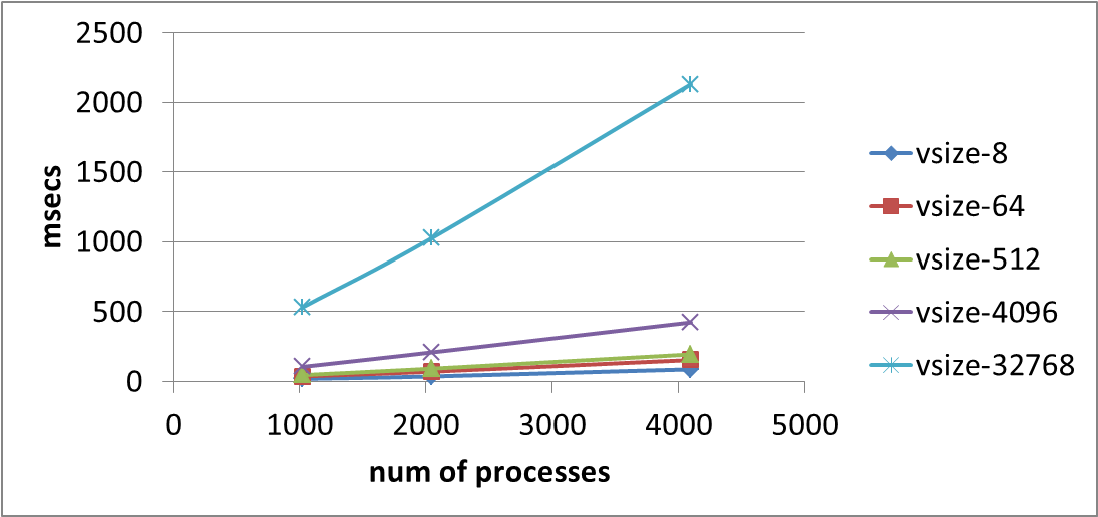
\includegraphics[width=.75\linewidth]{sync}
%  \label{fig:sync:noredund}
%}%
%\end{subfigure}
%\begin{subfigure}[Improvements with redundant values]{
%  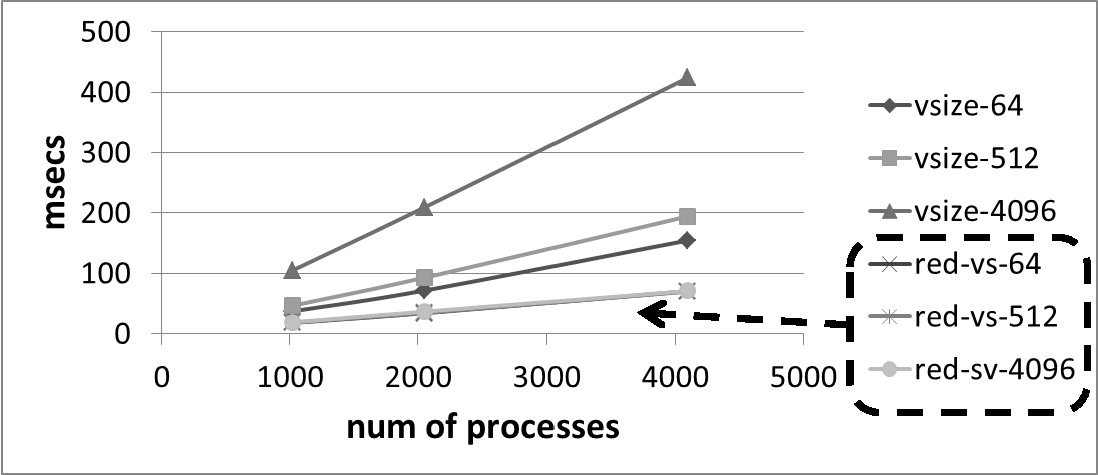
\includegraphics[width=.75\linewidth]{sync-redund}
%  \label{fig:sync:redund}
%}%
%\end{subfigure}
%\caption{Max latency of synchronization phase}
%\vspace{-.6cm}	
%\label{fig:sync}
%\end{figure}
%

\begin{figure}
\centering
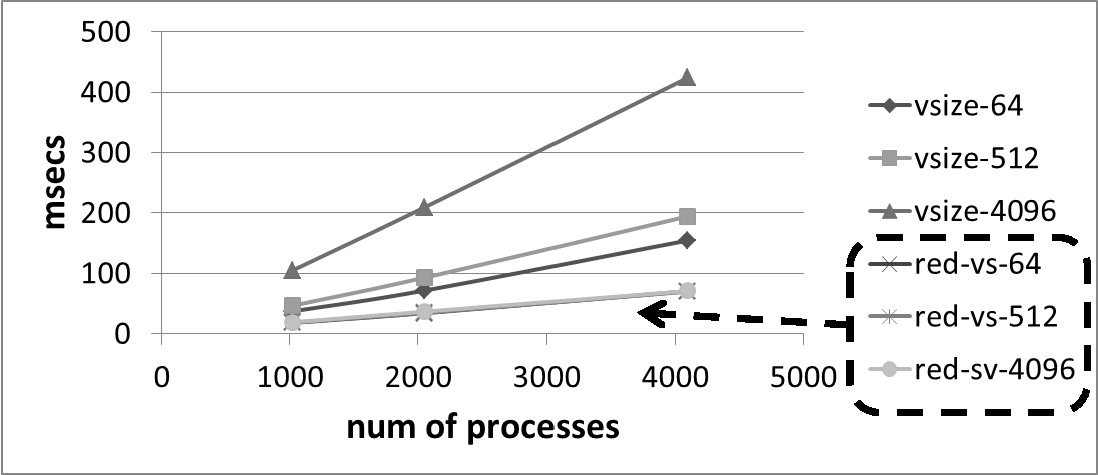
\includegraphics[width=1.0\linewidth]{sync-redund}
\caption{Max latency of synchronization phase}
\vspace{-.7cm}	
\label{fig:sync}
\end{figure}
 

Moving on to the synchronization phase, Figure~\ref{fig:sync} shows 
how {\tt kvs\_fence} scales as the number of producers increase. 
As with the producer latency,
each plot represents different value sizes under two different
value types: unique values vs. redundant values.
The most revealing observation is that
fence scalability depends on the level of
redundancy in key-value objects that had previously 
been put in. Figure~\ref{fig:sync} 
shows the improvements made when redundant values are used. 
Label {\tt red-vsize-k} is the maximum latency metric
as {\tt vsize-k} except that 
redundant values had been used.

We theorize that in the unique-value case, fence performs 
linearly with respect to the number of
producers because these values are simply being {\em concatenated} while
being sent up the tree, and that it performs logarithmically for the
redundant-value case
because redundant values are {\em reduced} while being sent 
up the tree. However, our data shows that the redundant-value case
falls short of logarithmic scaling, and we believe this is
because while values are reduced, the {\em (key, SHA1)} tuples
referring to them are still concatenated.

%\ifcomments
%\marginpar{\tiny DA: I am speculating a bit for redundant case; my job on cab will confirm or deny this.}
%\marginpar{\tiny JG: Dong I can't see any difference between
%\ref{fig:sync:redund} and \ref{fig:sync:noredund}.}
%\fi
%
\begin{figure}[ht]
\centering
\begin{subfigure}[With single-directory layout]{
  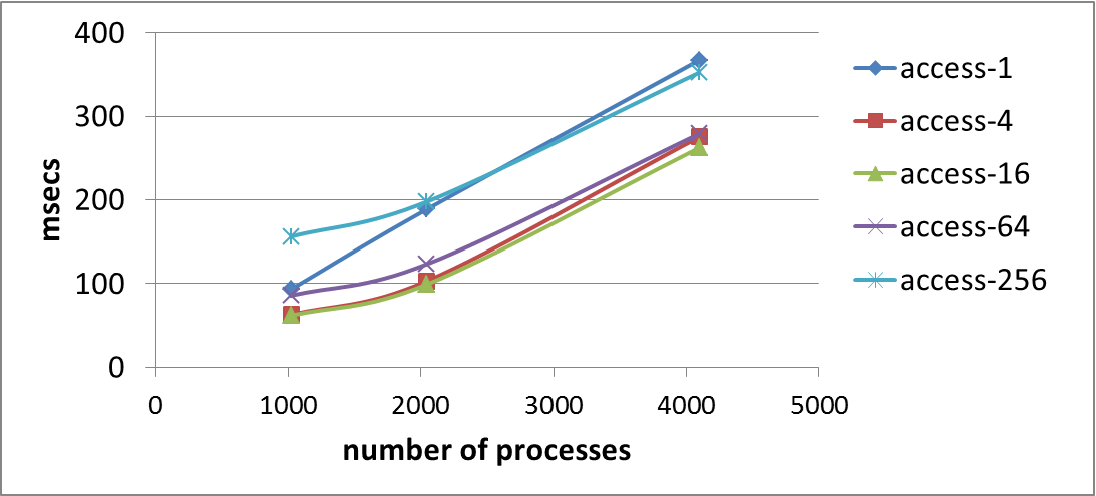
\includegraphics[width=1.0\linewidth]{consumer-1-dir}
  \label{fig:cons:dir}
}%
\end{subfigure}
\begin{subfigure}[Improvements with multiple directories]{
  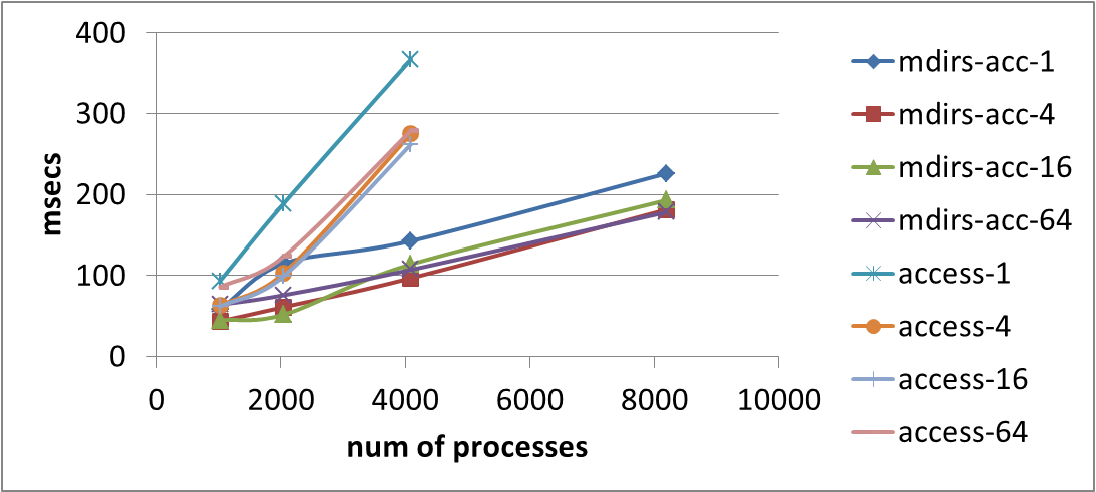
\includegraphics[width=1.0\linewidth]{consumer-dist-dir}
  \label{fig:cons:dirs}
}%
\end{subfigure}
\caption{Max latency of consumer phase (value size: 8 bytes)}
\vspace{-.3cm}
\label{fig:consumer}
\end{figure}

Next, Figure~\ref{fig:consumer} shows the maximum latency of the consumer
phase. % with respect to various parameter settings. 
These results show how {\tt kvs\_get}
scales as we increase the number of consumers. Each plot represents
the latency when each consumer reads different numbers of 
objects, e.g., the {\tt access-4} plot represents each consumer reading
4 distinct objects.  While these figures show only the performance of reading
objects 8 bytes in size, we observe that 
scalability trends are similar at different value sizes.
%Surprisingly, we see little change in performance when value sizes
%exceed the 42-byte store-by-reference limit.

Figure~\ref{fig:cons:dir} shows the maximum latency of {\tt kvs\_get}
when the target keys are all stored in a single
KVS directory object. The latency is quite high and also increases
linearly as we increase the number of consumers. 
It appears that the poor performance and scaling behavior 
are attributed to the fact that our slave caches store only full
objects, and the small objects being consumed in the test cannot
be retrieved without faulting in the entire directory object
containing them, through the tree of CMB slave cache instances.

With our access pattern where $G$ objects are read collectively by
$C$ consumers, and the time to replicate $G$ objects in a single slave cache
from its CMB-tree parent is given by $T(G)$, the maximum consumer latency is given by
\begin{equation}
log_2(C) \times T(G).
\end{equation}
Thus, the max latency increase for every doubling of consumers is
\begin{equation}
\frac{log_2(2C) \times T(2G)}{log_2(C) \times T(G)}.
\end{equation}
Generally, this would approach 2, 
as we continue to increase the number of consumers,
and our data match with this model.

We can improve this behavior by storing objects across multiple
directories. Slave caches can then operate at a finer granularity,
and the quantity of data that must be retrieved to satisfy consumer
requests will tend, depending on how requests stride directories,
to be proportional to the quantity of data requested.
This is especially true toward the leaves of the CMB tree where the
slave caches service a decreasing subset of consumers.
Figure~\ref{fig:cons:dirs} shows the improvements 
when objects are spread into directories of 128 objects each.
Label {\tt mdir-acc-k} refers to the same access pattern as {\tt access-k} 
except the objects are stored across multiple directories.

%\ifcomments
%\marginpar{\tiny JG: Dong, can \ref{fig:cons:dir} and \ref{fig:cons:dirs}
%be refactored for clarity so the first has access plots and the second
%has mdirs-acc plots?}
%\fi
When objects are spread across directories and the amount of data
faulted into slave caches decreases as a function of tree levels, 
the latency can be modeled as a geometric series.
For example, at tree height $h$, the latency would be 
\begin{equation}
T(G) + T(\frac{G}{2}) + T(\frac{G}{4}) + ... + T(\frac{G}{2^h}),
\end{equation}
where each term represents the latency of replication per level,
and the sum approaches $2T(G)$. Thus, its improvement over the single
directory scheme is on the order of 
\begin{equation}
\frac{log_2(C) \times T(G)}{2 T(G)} = \frac{1}{2}log_2(C).
\end{equation}
The improvements would be linearly 
greater as we increase the scale and our measurements agree with this. 

While these results suggest a promising avenue for reworking the KVS internal
object layout for performance, we note that such a scheme alone
would fall short of reaching extreme scale.
Our model suggests that the latency will grow linearly when $G$ grows
with the scale. For example, if $G$ doubles every time the number of
consumers is doubled, our geometric series model predicts the latency will
also double according to
\begin{equation}
\frac{2T(2G)}{2T(G)}.
\end{equation}
With the current scheme, the only way to gain true logarithmic
scaling is when $G$ stays constant regardless of scale. 
%MS: don't think this is true anymore
%In a later section, we will discuss some of our plans 
%to exploit the understanding we gained from the evaluation. 
